%!TEX root = ../thesis.tex
\section{緒言}
本章では、本研究での歩行パターン生成器の実装手法、及び公開した情報について述べる。

\section{公開する情報}
本研究では、公開する内容として、文献等で明文化されにくい部分を特に対象とする。現状、文献等での明文化が少ないと筆者が捉えているのは以下の3種の情報である。
\begin{enumerate}
  \item 具体的なソースコードの実装
  \item 実際に歩行パターンを生成可能なパラメータの例
  \item 実装時に得た知見
\end{enumerate}

以上3種の情報に対して、本研究では具体的に以下に示す情報を公開する。

\begin{itemize}
  \item C++言語で実装したMPCによる歩行パターン生成器のソースコード
  \item 式\eqref{eq:mpc_valuefunc}で示されるMPCの標準形である評価関数を最適化ソルバーが求める形式へ変形する手法
  \item 実装した歩行パターン生成器で歩行パターンを生成可能なパラメータの一例
  \item 上記の実装を行う上で、筆者が得た知見
\end{itemize}

上記をまとめ、インターネット上で誰でもアクセス可能なGithub\cite{MYGITHUB}にて情報の公開を行う。

\begin{figure}[hbtp]
  \centering
 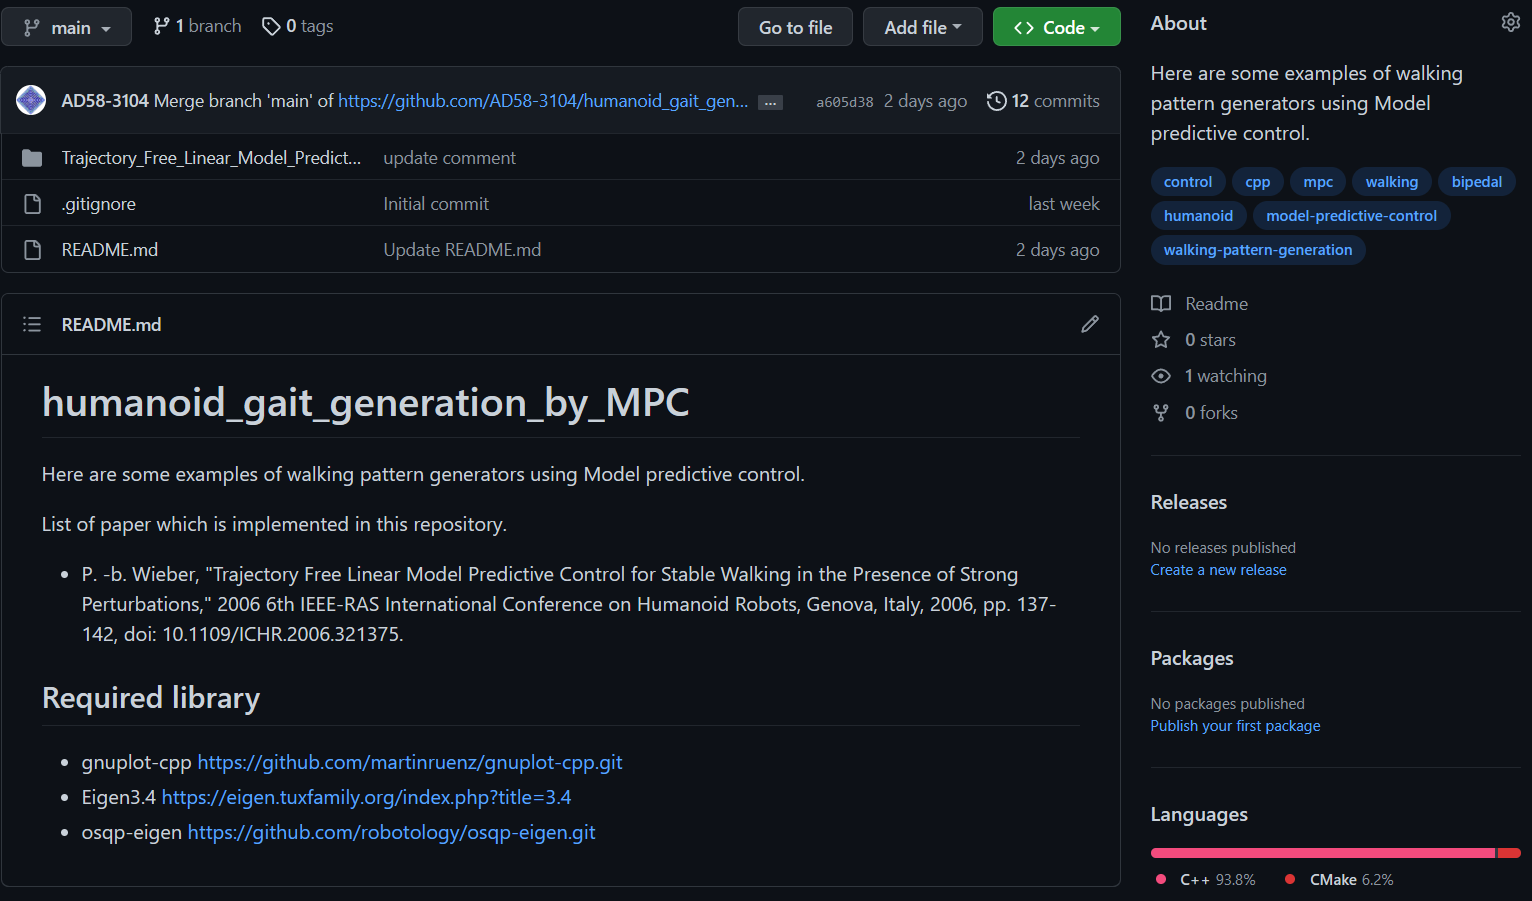
\includegraphics[keepaspectratio, scale=0.4]
      {images/github_example.png}
\caption{ Github page of publication}
 \label{Fig:github_example}
\end{figure}

\section{C++言語によるMPCを利用した歩行パターン生成器の実装}

本研究では、以下の\ref{tb:library}に示すライブラリ群を利用し、C++言語にて実装を行った。

\begin{table}[htbp]
  \centering
  \begin{tabular}{|c|c|} \hline
    QP solver              & osqp\cite{OSQP}            \\ \hline
    C++ binding of osqp    & osqp-eigen\cite{OSQPEIGEN} \\ \hline
    Linear algebra library & eigen-3.4.0\cite{EIGEN}    \\ \hline
  \end{tabular}
  \caption{Libraries used for implementation}
  \label{tb:library}
\end{table}


\section{実装上必要なMPCの式変形}
式\eqref{eq:control-general-system}で表される標準的なシステムに対する、MPCにおける評価関数の標準的な立式は式\eqref{eq:mpc_general_valuefunc}となる。

\begin{equation}
  \min_{{\buildrel\ldots\over{x}}_{k},{\buildrel\ldots\over{x}}_{k+1},\ldots,{\buildrel\ldots\over{x}}_{k+n}}\sum_{i=k}^{n}{1\over 2}Q\left(x_{i+1}-x_{i+1}^{ref}\right)^{2}+{1\over 2}R{u}_{i}^{2}
  \label{eq:mpc_general_valuefunc}
\end{equation}

また、制約は以下の様に表される。
(式を書く) 状態制約 不等式と等式
(式を書く) 入力制約 不等式と等式

ここで、MPCの評価関数の標準形である式\eqref{eq:mpc_general_valuefunc}をQPによって最小化する場合、MPCの等式、不等式制約を含め、QPの標準形となる式\eqref{eq:qp_standardform}の形に変形する必要が生じる。

\begin{equation}
  \underset{x}{\min} \frac{1}{2}x^TQx \;\;\; subject \; to \; Ax = b
  \label{eq:qp_standardform}
\end{equation}

特に、MPCの実装においては何らかのQPソルバーを利用する場合が多く、利用するソルバが求める形となるように評価関数(式())と制約(式())を変形する必要が生じる。
例として、matlab\cite{MATLAB:2021}のQPソルバであるquadprog\cite{MATLABQUADPLOG}では、以下の形式で表す必要がある。

\begin{equation}
  \underset{x}{\min} \frac{1}{2}x^THx + f^Tx
  \label{eq:qp_prog}
\end{equation}

\begin{equation}
  such \; that \;\;
  \begin{cases}
    A \cdot x \leq b,  \\
    Aeq \cdot x = beq, \\
    lb \leq x \leq ub.
  \end{cases}
  \label{eq:qp_constraint}
\end{equation}

ここで、$H,A,Aeq$は行列、$f,b,beq,lb,ub,x$はベクトルである。

また、今回利用したQPソルバであるosqp\cite{OSQP}もそれのPython、C、C++に向けたバインディング全てでmatlabのquadprogと同じく式\eqref{eq:qp_prog}と式\eqref{eq:qp_constraint}の形式で評価関数と制約を表現する必要がある。

この変形方法について述べる。

まず、評価関数を変形する。
これは、式\eqref{eq:mpc_valuefunc}を展開し、xに関する二次の項と、一次の項でまとめると以下の式\eqref{eq:mpc_to_qp}となる。これは、QPの標準形である式\eqref{eq:qp_prog}の形式である。

(式を入れる)
\begin{equation}
  J =  x^TQx - 2xQx_{ref} + Ru^2
  \label{eq:mpc_to_qp}
\end{equation}

次に、制約をQP形式である式\eqref{eq:qp_constraint}として表す。
ここで、MPCの制約条件である式()式()と式\eqref{eq:qp_constraint}を比較すると、MPCでの制約条件は状態(出力)と入力の二種の変数に対する制約であるのに対して、QPでは式\eqref{eq:qp_constraint}のようにQPの最適解であるベクトルxで表す。
ここで、ニ種の制約を式\eqref{eq:qp_constraint}の一つの行列Aで表すための実装上の工夫として、最適解であるxを拡張して、以下のように表現する。

\begin{equation}
  x =
  \begin{pmatrix}
    x_{k} \\ x_{k+1} \\ \vdots \\ x_{k+n}
    \\
    u_{k} \\ \vdots \\ u_{k+n}
  \end{pmatrix}
  \label{eq:augment_vec}
\end{equation}

ここで、xは出力、ないしは状態、xがQPの最適解(MPCにおける入力)とする。
式\eqref{eq:qp_prog},\eqref{eq:qp_constraint}のxを上記の式\eqref{eq:augment_vec}のベクトルで表すと、式\eqref{eq:qp_constraint}は以下のように表せる。

\begin{equation}
  A_{c} =
  \left(
  \begin{array}{ccccc|cccc}
      -I & 0 & 0 & \cdots & 0 & 0 & 0 & \cdots & 0 \\ A & -I & 0 & \cdots & 0 & B & 0 & \cdots & 0 \\ 0 & A & -I & \cdots & 0 & 0 & B & \cdots & 0\\ \vdots & \vdots & \vdots & \ddots & \vdots & \vdots & \vdots & \ddots & \vdots \\ 0 & 0 & 0 & \cdots & -I & 0 & 0 & \cdots & B\\ \hline I & 0 & 0 & \cdots & 0 & 0 & 0 & \cdots & 0\\ 0 & I & 0 & \cdots & 0 & 0 & 0 & \cdots & 0\\ 0 & 0 & I & \cdots & 0 & 0 & 0 & \cdots & 0\\ \vdots & \vdots & \vdots & \ddots & \vdots & \vdots & \vdots & \ddots & \vdots \\ 0 & 0 & 0 & \cdots & I & 0 & 0 & \cdots & 0\\ 0 & 0 & 0 & \cdots & 0 & I & 0 & \cdots & 0\\ 0 & 0 & 0 & \cdots & 0 & 0 & I & \cdots & 0\\ \vdots & \vdots & \vdots & \ddots & \vdots & \vdots & \vdots & \ddots & \vdots \\ 0 & 0 & 0 & \cdots & 0 & 0 & 0 & \cdots & I
    \end{array}
  \right)
  \label{eq:mpc_constraint_matrix}
\end{equation}

%  \f] while the upper and the lower bound are \f[ l = \begin{bmatrix} -x_0 \ 0 \ \vdots \ 0 \ x_{min}\ \vdots\ x_{min}\ u_{min}\ \vdots\ u_{min}\ \end{bmatrix} \quad u = \begin{bmatrix} -x_0 \ 0 \ \vdots \ 0 \ x_{max}\ \vdots\ x_{max}\ u_{max}\ \vdots\ u_{max}\ \end{bmatrix}


拡大ベクトルを使った表記、等式制約と不等式制約を適当にやる。

(式を書く)

\begin{equation}
  \begin{pmatrix}
    e_{0}\\
    \vdots \\
    e_{i}\\
    l_{0}\\
    \vdots\\
    l_{i}
  \end{pmatrix}
  \leq
  \begin{pmatrix}
    x_{k} \\ x_{k+1} \\ \vdots \\ x_{k+n}
    \\
    u_{k} \\ \vdots \\ u_{k+n}
  \end{pmatrix}
  \leq
  \begin{pmatrix}
    e_{0}\\
    \vdots\\
    e_{i}\\
    u_{0}\\
    \vdots\\
    u_{i}
  \end{pmatrix}
\end{equation}

式\eqref{eq:mpc_constraint_vectors}のuiは不等式制約の上限、liは不等式制約の下限、eiは等式制約の値とする。

ここで、Aの上部N列を構成する等式制約はモデル予測制御における有限長の未来の状態の予測である。この等式制約により、式()のzを状態予測値として束縛する。これにより、QPの形式でMPCの状態に関する制約を表現することが可能となる。また、この予測は、出力に対しても行うことができる。その場合は予測の式()に対してCの対角行列式()を左から掛ける。

最適解のベクトルを式\eqref{eq:augment_vec}の形式に拡大したことで、MPCの評価関数 式\eqref{eq:mpc_valuefunc}を展開し、ベクトルx~の二次の項と一次の項でまとめた式は以下となる。

(式を書く) hとgについて明示する


\section{本研究で実装したソフトウェアのパラメータ}

ここでは、4章に示す、本研究で実装したソフトウェアで歩行パターンを生成可能なパラメータについて解説する。

本研究で実装した歩行パターン生成手法では、主に表\ref{tb:parametor_list}がパラメータとして調整可能な要素とされる。

\begin{table}[htbp]
  \centering
  \begin{tabular}{|c|c|} \hline
    Control Horizon  [$s$] \\ \hline
    Unit time  [$ms$] \\ \hline
    Q / R   \\ \hline
    % Height of CoM  [$m$] \\ \hline
    Step width  [$m$] \\ \hline
    Upper bound of difference between ref and current output.  [$m$] \\ \hline
    Lower bound of difference between ref and current output.  [$m$] \\ \hline
    Upper bound of input  [$m/s^{3}$] \\ \hline
    Lower bound of input  [$m/s^{3}$] \\ \hline
  \end{tabular}
  \caption{Libraries used for implementation}
  \label{tb:parametor_list}
\end{table}

表\ref{tb:parametor_list}の要素のうち Control Horizon、Unit time、Q / R、Step widthは主に生成する歩行パターンの安定性、追従性能に影響を及ぼす。また、Control Horizon、Unit time、Q / R、Step widthに対する入力と出力の上下限の制約の関係は、解となる最適入力の実行可能性に影響を及ぼす。
本研究の中で、情報としてGithub\cite{MYGITHUB}で公開した表\ref{tb:parametor_list}に示したパラメータの具体的例は4章で示す。